% Everything that comes from theory and that is needed to understand and describe our work.
	\subsection{802.11} \label{theory:prot_specs}
	802.11 is the standard family of protocols for wireless networks. It is also named Wi-Fi. Protocols in the 802.11 family describe how various wireless devices must interact. There are two kinds of wireless networks: BSS and IBSS.
	\begin{description}
		\item[BSS (infrastructure)] is a centralized network, in this case we have one or more AP (Access Point) and various clients (STAs) can access to the network throw it.
		\item[IBSS (ad-hoc)] is a sample client to client (STA to STA) network.
	\end{description}
	Nowadays the most popular (and commercial) 802.11 implementations are 802.11b and 802.11g.
	
% A simple description of how an IEEE 802.11 protocol works to introduce the fact that there is some overhead added by the protocol.
% Yes, I know it's unbelivable but there are some differences, for real! :)
	\subsection{Differences between 802.11b and 802.11g} \label{theory:prot_differences}
	
	The 802.11b protocol was born in October 1999, and since then it has a discrete success.  However, later on some other wireless devices, such as cordless telephones, use the same frequencies and therefore produce interferences with 802.11b-conforming devices and cause slower performance of these.
	% As a consequence,
	802.11b extends the basic net bit rate of the standard 802.11 up to 11 Mbit/s.\\
	
	In June 2003 arrives 802.11g, which is fully backwards compatible with 802.11b, but brings better bit rates and throughput\\
	
	Both protocols use the same frequency band (2.4 GHz), but different frequency spreads.
	
	\begin{table}[h]
		
		\begin{tabularx}{15cm}{ | X X X X X X | }
			\hline
				802.11 Protocol & Release & Frequency (GHz) & Typical throughput (Mbit/s) & Maximal net bitrate (Mbit/s) & Modulation \\
			\hline
				-- & Jun 1997 & 2.4 & 00.9 & 002 & DSSS \\
				b & Sep 1999 & 2.4 & 04.3 & 011 & DSSS \\
				g & Jun 2003 & 2.4 & 19 & 054 & OFDM \\
			\hline
		\end{tabularx}
		
		\caption{802.11 family standard}
		\label{802.11_family_standard}
	\end{table}
	
	% TODO: ``shy of fivefold then'' ???????
	%As we can see from the table the standard 802.11g's typical throughput is just shy of fivefold then 802.11b standard typical throughput and the main difference is the modulation method. While 802.11b use direct sequence spread spectrum signaling (DSSS), 802.11g use orthogonal frequency division multiplexing (OFDM) methods. Because of OFDM, 802.11g increases the net bit rate up tu 54 Mbit/s.
	%rewrite:
	As we can see from the table, the 802.11g standard's typical throughput is five times that of 802.11b's typical throughput.  The main difference is the modulation method.  While 802.11b uses direct sequence spread spectrum signalling (DSSS), 802.11g uses orthogonal frequency division multiplexing (OFDM) instead.  Because of OFDM, 802.11g increases the net bit rate to up to 54 Mbit/s.
	
	\begin{itemize}
		\item 802.11b (DSSS)
			\begin{description}
				\item[Modulation DBPSK, DQPSK] 1 and 2 Mbit/s
				\item[Modulation CCK] 5.5, 11 Mbit/s
			\end{description}
		\item 802.11g (OFDM)
			\begin{description}
				\item[Modulation BPSK, QPSK, 16QAM, 64QAM] 6, 9, 12, 18, 24, 36, 48, 54 Mbit/s
			\end{description}
	\end{itemize}

	% REWRITTEN  When a 802.11g device communicates with a 802.11b device it uses, in order to retrocomputability, DSSS  so it go down with DSSS speeds.
	% TODO check, please:
	When an 802.11g device communicates with an 802.11b device, it switches back to DSSS for backward compatibility. As a consequence, it must communicate with the slower speed of DSSS.

	However more important than the physical throughput is the effective throughput, which is always lower in relation to the nominal bit rate.
	In 802.11b, we can have a typical throughput of 4,3 Mbit/s over a 11 Mbit/s of channel capacity while in 802.11g we have a typical throuughput of 25 Mbit/s over a 54 Mbit/s of channel capacity. This is due to the overhead of the communication.
	
	The 802.11 standard basically defines two layers, a physical layer (PHY) and a media access control layer (MAC). To understand the reason behind the different throughputs, we have to analyze the MAC Frame Format (Figure \ref{mac_packet}).
	
	\begin{figure}[h!]
		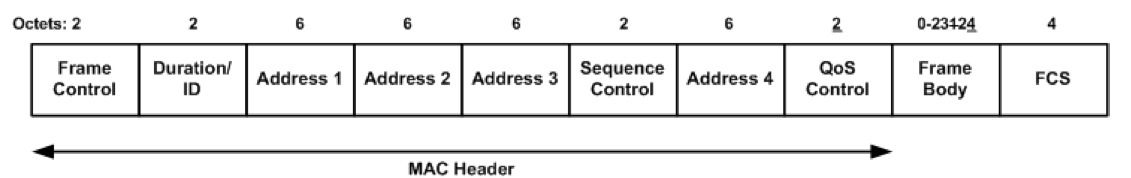
\includegraphics[angle=0, keepaspectratio=true, width=15cm]{../images/mac_header2}
		\caption{MAC Frame Format}
		\label{mac_packet}
	\end{figure}
	
	% TODO: ``need to WEP and MSDU'' ?????
	The total header cost in terms of bytes is fixed to 32 bytes (octets) over a variable size of the frame body from 0 to 2304 bytes plus any overhead from security encapsulation. The frame body size is determined by the maximum MSDU + ICV + IV, where ICV (Integrity Check Value) and IV (Initialization Vector) need to WEP and MSDU is the Mac Service Data Unit. Therefore the real throughput depends by frame body length.\\
	
    % TODO inserti missing figure
    % \begin{figure}[h!]
    %   \includegraphics[angle=0, keepaspectratio=true, width=15cm]{../images/ppdu_frame_format}
    %   \caption{PPDU Frame Format}
    %   \label{ppdu_frame_packet}
    % \end{figure}
	
	To calculate the theoretical throughput with a DATA size of 1470 bit we have to follow the two formulas written below:
	
	\begin{gather*}
		\textrm{Throughput}_{phys} = \\\\
		= \frac{ ( \textrm{DATA}_{bit} + \textrm{HEADER IP}_{bit} + \textrm{HEADER UDP}_{bit} + \textrm{HEADER MAC}_{bit} ) \times 8 }{ \textrm{FRAME}_{seconds} } = \\\\
		= \frac{ 1532 \times 8 }{  \textrm{FRAME}_{seconds} } \\\\
	\end{gather*}
	
	\begin{gather*}
		\textrm{Throughput}_{UDP} = \frac{ \textrm{DATA}_{bit} \times 8 }{ \textrm{FRAME}_{seconds} } = \frac{ 1470 \times 8 }{  \textrm{FRAME}_{seconds} } \\\\
	\end{gather*}
	
	Table \ref{tbl:80211bgexample} shows an example theoretical throughput of the two standards at two different speeds.
	
	\begin{table}[h!]
		\begin{tabularx}{15cm}{ | X | X | X | X | X | }
			\hline
				 & \multicolumn{2}{|c|}{ 802.11b (DSSS)} & \multicolumn{2}{|c|}{ 802.11g-only (OFDM)} \\
				 \hline
				 & 5.5 Mbit/s & 11 Mbit/s & 6 Mbit/s & 54 Mbit/s \\
			\hline
				DIFS & 50 $\mu$s & 50 $\mu$s & 28 $\mu$s & 28 $\mu$s \\
			\hline
				SIFS & 10 $\mu$s & 10 $\mu$s & 10 $\mu$s & 10 $\mu$s \\
			\hline
				CW & 310 $\mu$s & 310 $\mu$s & 139.5 $\mu$s & 139.5 $\mu$s \\
			\hline
				PLPC Preamble + PLPC Header & 96 $\mu$s & 96 $\mu$s & 26 $\mu$s & 26 $\mu$s \\
			\hline
				MAC Header + LLC & 52.36 $\mu$s & 26.18 $\mu$s & 48 $\mu$s & 5.33 $\mu$s \\
			\hline
				IP + UDP Headers & 40.73 $\mu$s & 20.36 $\mu$s & 37.33 $\mu$s & 4.15 $\mu$s \\
			\hline
				Data (1470 byte)& 2138.18 $\mu$s & 1069.09 $\mu$s & 1960 $\mu$s & 217.78 \\
			\hline
				TAIL DATA & -- & -- & 1 $\mu$s & 0.11 $\mu$s \\
			\hline
				ACK PLPC Preamble + Header & 96 $\mu$s & 96 $\mu$s & 26 $\mu$s & 26 $\mu$s \\
			\hline
				ACK & 20.36 $\mu$s & 10.18 $\mu$s & 18.67 $\mu$s & 2.07 $\mu$s \\
			\hline
				TAIL ACK & -- & -- & 1 $\mu$s & 0.25 $\mu$s \\
			\hline
			\hline
				TOTAL & 2813.63 $\mu$s & 1687.81$\mu$s & 2295.5 $\mu$s & 459.19 $\mu$s \\
			\hline
			\hline
				Theoretical physical throughput & 4.35 Mbit/s $\mu$s & 7.26 Mbit/s & 5.33 Mbit/s & 26.69 Mbit/s \\
			\hline
			\hline
				Theoretical physical throughput UDP & 4.17 Mbit/s & 6.96 Mbit/s & 5.12 Mbit/s & 25.61 Mbit/s \\
			\hline
			
		\end{tabularx}
		\caption{Example theoretical throughput for 802.11b and 802.11g}
		\label{tbl:80211bgexample}
	\end{table}
	
	
	\subsection{Fragmentation Threshold and RTS Threshold} \label{theory:frag_rts}
	
	802.11, in order to improve the performance, allows to adjust some parameters like Frag (Fragmentation Threshold) and RTS/CTS (Request To Send / Clear To Send).
	
	\begin{description}
		\item[Fragmentation Threshold] is a technique witch divide a big packet into many small packets. These small packets can be transmitted more quickly into the medium (the air). On the one hand this technique works great avoid the collision but on the other hand it increase the overhead because of the packets header. The possible values range is from 256 to 2346.
	
		\item[RTS Threshold] is the frame size above which an RTS/CTS handshake will be performed before attempting to transmit. The possible values range is from 256 to 2346.
	
		\item[RTS/CTS] is a control signal witch try to synchronize the communication. When a device send an RTS (Request To Send) signal this mean that it is ready to send data, in particular RTS/CTS asks for permission to transmit to reduce collisions, but adds considerable overhead. Disabling RTS/CTS can reduce overhead and latency in WLANs where all stations are close together, but can increase collisions and degrade performance in WLANs where stations are far apart and unable to sense each other to avoid collisions (``Hidden Nodes'', ``Hidden Terminal'').
	\end{description}

% Calculate protocols upperbound limitations and similar things (report the formulas!).
% DO NOT USE PROFESSOR SLIDES AS SOURCE OF INFORMATIONS SINCE MOST OF VALUES ARE COMPLETELY WRONG!!!!!!!!!
% Download the IEEE standard from here: http://disi.unitn.it/locigno/didattica/NC/802.11-2007.pdf and make a large use of ^F.

	








